\section{Bienvenidos al Diseño del Videojuego}


La joven protagonista despierta de una pesadilla en una habitación dentro de una casa gigante. Al mirar a su alrededor no reconoce la habitación. A pesar de su confusión, miedo y tristeza por estar sola en un lugar desconocido se arma de valor y decide avanzar recolectando objetos que la ayudaran a librarse de los monstruos y avanzar por la casa.\newline
\newline

A medida que avanza por la casa se dará cuenta de que los objetos y monstruos se parecen mucho a los juguetes con los que jugaba con su hermano a "Monstruos y brujas". Pero no te confíes, los monstruos de la casa serán cada vez más feroces y más difícil de matar y deberás mejorar tus técnicas conseguir mejores objetos.\newline
\newline

\centerline{¡Ayúdala a llegar hasta el final y conseguir escapar de ese horrible lugar!}


\section{Objetivo del juego}

Deberás ayudar a protagonista a avanzar por las distintas habitaciones derrotando monstruos, conseguir mejores objetos, descubrir como has llegado hasta allí y lo mas importante, conseguir ser feliz de nuevo.

\section{Clasificación del tipo de juego}

Este juego es del género RPG y va orientado a las niñas jóvenes de entre 10 y 15 años según se especificó en los requerimientos del proyecto a realizar. Entendemos según la investigación que hemos llevado a cabo, preguntando a hermanas, amigas, buscando por internet tendencias de videojuegos que juegan las chicas con esa franja de edad, que los juegos que más se juegan no dependen tanto del género, si no de la edad del jugador. Por lo tanto debemos intentar que los recursos gráficos se adapten lo más posible a esta franja de edad. Para tratar de acercarnos más a los requerimientos del juego tenemos pensado que el personaje principal sea una niña de edad similar para que así los niñas a las cuales va dirigido nuestro juego se sientas más identificadas con la protagonista.

\newpage

\section{Historia del personaje principal}

El juego comienza con la protagonista despertando en una pesadilla, se encuentra en una casa gigante desconocida, está triste, asustada y confundida. El cuarto en el que está no le es familiar, sin embargo, investigando el lugar se da cuenta de que los objetos que hay desperdigados por los diferentes lugares sí, ¡son sus juguetes!

\begin{figure}[!htb]
  \centering
    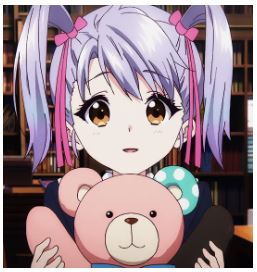
\includegraphics[width=0.5\linewidth]{./img/child.JPG}
    \caption{Idea de personaje principal.}
  \label{fig:yo}
\end{figure}
\newline
De repente, escucha de fondo unos ruidos espantosos que provienen de un cuarto, lentamente se va acercando a él y ve a un monstruo. Al principio se asustó, pero tras breves instantes le pareció extrañamente familiar, se parece mucho a una figurita de juguete de su hermano, ¡Pero este está vivo! \newline
\newline
Recordó que hace pocos días estuvo jugando con su hermano a “Monstruos y Brujas” y ella siempre conseguía matar al monstruo de su hermano con un juguete en específico… \newline
\newline
Un momento, ¡es el objeto que encontró en el cuarto en el que despertó! Se armó de valor, entró al cuarto, y con el objeto derrotó al monstruo.

\section{Cámara del jugador y controles}

La cámara queremos que sea de tipo Top-down ya que consideramos que es la más óptima para los juegos del género rpg. Además, los mapas están creados con Tiles por lo que será será mas fácil moverse y explorar las habitaciones. De forma adicional, el hecho de elegir este tipo de cámara nos va a reportar el no implementar los saltos, por lo que la complejidad de la programación será menor, y la demanda de CPU también.
\newpage

\begin{figure}[!htb]
  \centering
    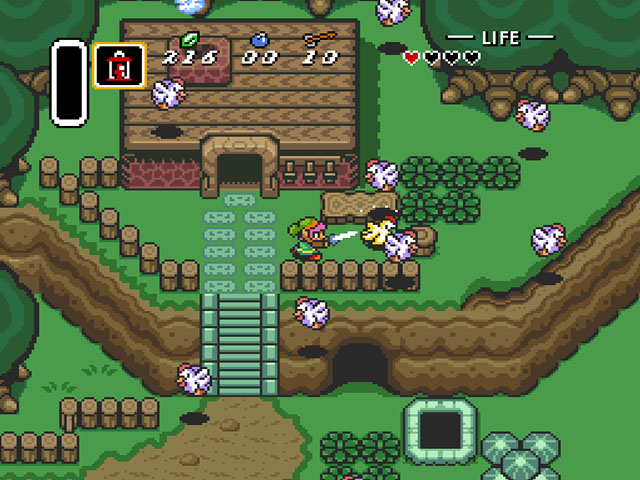
\includegraphics[width=\linewidth]{./img/camara.jpg}
    \caption{Tipo de perspectiva de cama.}
  \label{fig:yo}
\end{figure}
En cuanto a los controles, hemos pensado que al ser un juego orientado a PC, los controles deben poder realizarse únicamente mediante teclado, ya que en el caso de que alguien quiera probar nuestro juego, pero solo disponga de un portátil, permitirle jugar. De esta manera queremos hacer el juego sea lo más independiente del hardware posible, para así abrir más el abanico de potenciales jugadores.

\section{Interfaz de usuario}
En cuanto al HUD el jugador deberá ver, la vida que aparece en forma de corazones en la zona superior. Además, queremos implementar un inventario que contenga de las cinco pociones posibles(vida, experiencia, fuerza, velocidad y dureza por ejemplo) en la zona inferior de la pantalla. Queremos hacer algo similar al inventario de Minecraft, sencillo y no es abusivo en pantalla.

\begin{figure}[!htb]
  \centering
    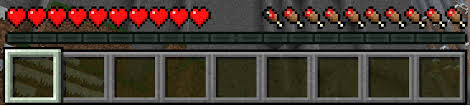
\includegraphics[width=\linewidth]{./img/barra.jpg}
    \caption{Tipo de HUD a implementar.}
  \label{fig:yo}
\end{figure}
\newpage
\section{Música y gráficos}
Al ser un grupo no mixto, somos todos estudiantes de ingeniería, y solo dos de nosotros tenemos cualidades de diseño gráfico básico, los recursos gráficos se tomarán de paginas de arte libre. Trataremos de crear los sprites básicos como son inventario, HUD, botones, pero los SpritesSheets de los mapas se tomarán de Internet referenciandolo y dando el mérito a los creadores de dichos recursos. De forma completamente análoga con el audio.\newline
\newline
Las herramientas utilizadas para el montaje y edición de los fondos y sprites han sido Photoshop, Gimp y Tiledmap. Photoshop y Gimp se ha utilizado para la edición de los fondos y Tiledmap se ha utilizado para la creación de los mapas. Se ha utilizado el programa WavePad para recortar algunos sonidos.



